% Options for packages loaded elsewhere
\PassOptionsToPackage{unicode}{hyperref}
\PassOptionsToPackage{hyphens}{url}
%
\documentclass[
]{article}
\usepackage{amsmath,amssymb}
\usepackage{iftex}
\ifPDFTeX
  \usepackage[T1]{fontenc}
  \usepackage[utf8]{inputenc}
  \usepackage{textcomp} % provide euro and other symbols
\else % if luatex or xetex
  \usepackage{unicode-math} % this also loads fontspec
  \defaultfontfeatures{Scale=MatchLowercase}
  \defaultfontfeatures[\rmfamily]{Ligatures=TeX,Scale=1}
\fi
\usepackage{lmodern}
\ifPDFTeX\else
  % xetex/luatex font selection
\fi
% Use upquote if available, for straight quotes in verbatim environments
\IfFileExists{upquote.sty}{\usepackage{upquote}}{}
\IfFileExists{microtype.sty}{% use microtype if available
  \usepackage[]{microtype}
  \UseMicrotypeSet[protrusion]{basicmath} % disable protrusion for tt fonts
}{}
\makeatletter
\@ifundefined{KOMAClassName}{% if non-KOMA class
  \IfFileExists{parskip.sty}{%
    \usepackage{parskip}
  }{% else
    \setlength{\parindent}{0pt}
    \setlength{\parskip}{6pt plus 2pt minus 1pt}}
}{% if KOMA class
  \KOMAoptions{parskip=half}}
\makeatother
\usepackage{xcolor}
\usepackage[margin=2in]{geometry}
\usepackage{color}
\usepackage{fancyvrb}
\newcommand{\VerbBar}{|}
\newcommand{\VERB}{\Verb[commandchars=\\\{\}]}
\DefineVerbatimEnvironment{Highlighting}{Verbatim}{commandchars=\\\{\}}
% Add ',fontsize=\small' for more characters per line
\usepackage{framed}
\definecolor{shadecolor}{RGB}{248,248,248}
\newenvironment{Shaded}{\begin{snugshade}}{\end{snugshade}}
\newcommand{\AlertTok}[1]{\textcolor[rgb]{0.94,0.16,0.16}{#1}}
\newcommand{\AnnotationTok}[1]{\textcolor[rgb]{0.56,0.35,0.01}{\textbf{\textit{#1}}}}
\newcommand{\AttributeTok}[1]{\textcolor[rgb]{0.13,0.29,0.53}{#1}}
\newcommand{\BaseNTok}[1]{\textcolor[rgb]{0.00,0.00,0.81}{#1}}
\newcommand{\BuiltInTok}[1]{#1}
\newcommand{\CharTok}[1]{\textcolor[rgb]{0.31,0.60,0.02}{#1}}
\newcommand{\CommentTok}[1]{\textcolor[rgb]{0.56,0.35,0.01}{\textit{#1}}}
\newcommand{\CommentVarTok}[1]{\textcolor[rgb]{0.56,0.35,0.01}{\textbf{\textit{#1}}}}
\newcommand{\ConstantTok}[1]{\textcolor[rgb]{0.56,0.35,0.01}{#1}}
\newcommand{\ControlFlowTok}[1]{\textcolor[rgb]{0.13,0.29,0.53}{\textbf{#1}}}
\newcommand{\DataTypeTok}[1]{\textcolor[rgb]{0.13,0.29,0.53}{#1}}
\newcommand{\DecValTok}[1]{\textcolor[rgb]{0.00,0.00,0.81}{#1}}
\newcommand{\DocumentationTok}[1]{\textcolor[rgb]{0.56,0.35,0.01}{\textbf{\textit{#1}}}}
\newcommand{\ErrorTok}[1]{\textcolor[rgb]{0.64,0.00,0.00}{\textbf{#1}}}
\newcommand{\ExtensionTok}[1]{#1}
\newcommand{\FloatTok}[1]{\textcolor[rgb]{0.00,0.00,0.81}{#1}}
\newcommand{\FunctionTok}[1]{\textcolor[rgb]{0.13,0.29,0.53}{\textbf{#1}}}
\newcommand{\ImportTok}[1]{#1}
\newcommand{\InformationTok}[1]{\textcolor[rgb]{0.56,0.35,0.01}{\textbf{\textit{#1}}}}
\newcommand{\KeywordTok}[1]{\textcolor[rgb]{0.13,0.29,0.53}{\textbf{#1}}}
\newcommand{\NormalTok}[1]{#1}
\newcommand{\OperatorTok}[1]{\textcolor[rgb]{0.81,0.36,0.00}{\textbf{#1}}}
\newcommand{\OtherTok}[1]{\textcolor[rgb]{0.56,0.35,0.01}{#1}}
\newcommand{\PreprocessorTok}[1]{\textcolor[rgb]{0.56,0.35,0.01}{\textit{#1}}}
\newcommand{\RegionMarkerTok}[1]{#1}
\newcommand{\SpecialCharTok}[1]{\textcolor[rgb]{0.81,0.36,0.00}{\textbf{#1}}}
\newcommand{\SpecialStringTok}[1]{\textcolor[rgb]{0.31,0.60,0.02}{#1}}
\newcommand{\StringTok}[1]{\textcolor[rgb]{0.31,0.60,0.02}{#1}}
\newcommand{\VariableTok}[1]{\textcolor[rgb]{0.00,0.00,0.00}{#1}}
\newcommand{\VerbatimStringTok}[1]{\textcolor[rgb]{0.31,0.60,0.02}{#1}}
\newcommand{\WarningTok}[1]{\textcolor[rgb]{0.56,0.35,0.01}{\textbf{\textit{#1}}}}
\usepackage{graphicx}
\makeatletter
\newsavebox\pandoc@box
\newcommand*\pandocbounded[1]{% scales image to fit in text height/width
  \sbox\pandoc@box{#1}%
  \Gscale@div\@tempa{\textheight}{\dimexpr\ht\pandoc@box+\dp\pandoc@box\relax}%
  \Gscale@div\@tempb{\linewidth}{\wd\pandoc@box}%
  \ifdim\@tempb\p@<\@tempa\p@\let\@tempa\@tempb\fi% select the smaller of both
  \ifdim\@tempa\p@<\p@\scalebox{\@tempa}{\usebox\pandoc@box}%
  \else\usebox{\pandoc@box}%
  \fi%
}
% Set default figure placement to htbp
\def\fps@figure{htbp}
\makeatother
\setlength{\emergencystretch}{3em} % prevent overfull lines
\providecommand{\tightlist}{%
  \setlength{\itemsep}{0pt}\setlength{\parskip}{0pt}}
\setcounter{secnumdepth}{-\maxdimen} % remove section numbering
\usepackage{geometry}
\usepackage{bookmark}
\IfFileExists{xurl.sty}{\usepackage{xurl}}{} % add URL line breaks if available
\urlstyle{same}
\hypersetup{
  pdftitle={Distribución Uniforme y Teorema Central del Límite},
  pdfauthor={Luz Alba Posse \& Martina Monastra},
  hidelinks,
  pdfcreator={LaTeX via pandoc}}

\title{Distribución Uniforme y Teorema Central del Límite}
\author{Luz Alba Posse \& Martina Monastra}
\date{2024-08-26}

\begin{document}
\maketitle

\section{Ejercicio 1: Distribución
Uniforme}\label{ejercicio-1-distribuciuxf3n-uniforme}

Sea \(X \sim U(0, 18)\) una variable distribuida uniformemente entre 0 y
18.

\subsection{1.a Generar la función
X\_dist(R)}\label{a-generar-la-funciuxf3n-x_distr}

\begin{Shaded}
\begin{Highlighting}[]
\FunctionTok{set.seed}\NormalTok{(}\DecValTok{6803}\NormalTok{)}

\CommentTok{\# 1.a Generar la función X\_dist(R)}
\NormalTok{X\_dist }\OtherTok{\textless{}{-}} \ControlFlowTok{function}\NormalTok{(R) \{}
  \FunctionTok{runif}\NormalTok{(R, }\AttributeTok{min =} \DecValTok{0}\NormalTok{, }\AttributeTok{max =} \DecValTok{18}\NormalTok{)}
\NormalTok{\}}
\end{Highlighting}
\end{Shaded}

\subsection{\texorpdfstring{1.b Calcular la media y la varianza muestral
de los datos para
\(R \in \{2, 30, 100, 10^4\}\).}{1.b Calcular la media y la varianza muestral de los datos para R \textbackslash in \textbackslash\{2, 30, 100, 10\^{}4\textbackslash\}.}}\label{b-calcular-la-media-y-la-varianza-muestral-de-los-datos-para-r-in-2-30-100-104.}

\begin{Shaded}
\begin{Highlighting}[]
\NormalTok{R\_values }\OtherTok{\textless{}{-}} \FunctionTok{c}\NormalTok{(}\DecValTok{2}\NormalTok{, }\DecValTok{30}\NormalTok{, }\DecValTok{100}\NormalTok{, }\DecValTok{10}\SpecialCharTok{\^{}}\DecValTok{4}\NormalTok{)}
\NormalTok{resultados }\OtherTok{\textless{}{-}} \FunctionTok{data.frame}\NormalTok{(}\AttributeTok{R =} \FunctionTok{integer}\NormalTok{(), }\AttributeTok{Media =} \FunctionTok{numeric}\NormalTok{(), }\AttributeTok{Varianza =} \FunctionTok{numeric}\NormalTok{())}

\ControlFlowTok{for}\NormalTok{ (R }\ControlFlowTok{in}\NormalTok{ R\_values) \{}
\NormalTok{  muestras }\OtherTok{\textless{}{-}} \FunctionTok{X\_dist}\NormalTok{(R)}
\NormalTok{  media\_muestral }\OtherTok{\textless{}{-}} \FunctionTok{mean}\NormalTok{(muestras)}
\NormalTok{  varianza\_muestral }\OtherTok{\textless{}{-}} \FunctionTok{var}\NormalTok{(muestras)}
\NormalTok{  resultados }\OtherTok{\textless{}{-}} \FunctionTok{rbind}\NormalTok{(resultados, }\FunctionTok{data.frame}\NormalTok{(}\AttributeTok{R =}\NormalTok{ R, }\AttributeTok{Media =}\NormalTok{ media\_muestral, }\AttributeTok{Varianza =}\NormalTok{ varianza\_muestral))}
\NormalTok{\}}

\FunctionTok{print}\NormalTok{(resultados)}
\end{Highlighting}
\end{Shaded}

\begin{verbatim}
##       R    Media  Varianza
## 1     2 3.377748  2.501266
## 2    30 8.270044 28.293709
## 3   100 8.220039 22.866303
## 4 10000 9.014883 27.267318
\end{verbatim}

\subsection{\texorpdfstring{1.c Calcular el valor teórico de la
esperanza de \(X\), \(E(X)\), y su varianza, \(V(X)\). Comparar estos
valores con los obtenidos en
1.b.}{1.c Calcular el valor teórico de la esperanza de X, E(X), y su varianza, V(X). Comparar estos valores con los obtenidos en 1.b.}}\label{c-calcular-el-valor-teuxf3rico-de-la-esperanza-de-x-ex-y-su-varianza-vx.-comparar-estos-valores-con-los-obtenidos-en-1.b.}

Teóricamente, para una distribución uniforme \(U(a, b)\), la esperanza
\(E(X)\) y la varianza \(V(X)\) se calculan como:

\[
E(X) = \frac{a + b}{2}, \quad V(X) = \frac{(b - a)^2}{12}
\]

En nuestro caso:

\begin{Shaded}
\begin{Highlighting}[]
\NormalTok{a }\OtherTok{\textless{}{-}} \DecValTok{0}
\NormalTok{b }\OtherTok{\textless{}{-}} \DecValTok{18}
\NormalTok{E\_X }\OtherTok{\textless{}{-}}\NormalTok{ (a }\SpecialCharTok{+}\NormalTok{ b) }\SpecialCharTok{/} \DecValTok{2}
\NormalTok{V\_X }\OtherTok{\textless{}{-}}\NormalTok{ (b }\SpecialCharTok{{-}}\NormalTok{ a)}\SpecialCharTok{\^{}}\DecValTok{2} \SpecialCharTok{/} \DecValTok{12}

\FunctionTok{print}\NormalTok{(}\FunctionTok{paste}\NormalTok{(}\StringTok{"Esperanza E(X):"}\NormalTok{, E\_X))}
\end{Highlighting}
\end{Shaded}

\begin{verbatim}
## [1] "Esperanza E(X): 9"
\end{verbatim}

\begin{Shaded}
\begin{Highlighting}[]
\FunctionTok{print}\NormalTok{(}\FunctionTok{paste}\NormalTok{(}\StringTok{"Varianza V(X):"}\NormalTok{, V\_X))}
\end{Highlighting}
\end{Shaded}

\begin{verbatim}
## [1] "Varianza V(X): 27"
\end{verbatim}

Al comparar con los valores muestrales obtenidos en 1.b, vemos que:

\begin{itemize}
\tightlist
\item
  La media muestral se acerca bastante al valor teórico de \(E(X)\).
\item
  La varianza muestral también se aproxima al valor teórico,
  especialmente cuando \(R\) es grande.
\end{itemize}

\subsection{\texorpdfstring{1.d Hacer dos histogramas de \(X\), tomando
\(R \in \{100, 10^4\}\) realizaciones y 30
bines.}{1.d Hacer dos histogramas de X, tomando R \textbackslash in \textbackslash\{100, 10\^{}4\textbackslash\} realizaciones y 30 bines.}}\label{d-hacer-dos-histogramas-de-x-tomando-r-in-100-104-realizaciones-y-30-bines.}

\begin{Shaded}
\begin{Highlighting}[]
\FunctionTok{par}\NormalTok{(}\AttributeTok{mfrow =} \FunctionTok{c}\NormalTok{(}\DecValTok{1}\NormalTok{, }\DecValTok{2}\NormalTok{))  }\CommentTok{\# Configurar la ventana gráfica para dos gráficos lado a lado}
\FunctionTok{par}\NormalTok{(}\AttributeTok{mar =} \FunctionTok{c}\NormalTok{(}\DecValTok{4}\NormalTok{, }\DecValTok{4}\NormalTok{, }\DecValTok{2}\NormalTok{, }\DecValTok{1}\NormalTok{))  }\CommentTok{\# Ajustar los márgenes del gráfico}

\CommentTok{\# Histograma para R = 100}
\FunctionTok{hist}\NormalTok{(}\FunctionTok{X\_dist}\NormalTok{(}\DecValTok{100}\NormalTok{), }\AttributeTok{breaks =} \DecValTok{30}\NormalTok{, }\AttributeTok{main =} \StringTok{"Histograma para X (R = 100)"}\NormalTok{, }\AttributeTok{xlab =} \StringTok{"Valores de X"}\NormalTok{, }\AttributeTok{col =} \StringTok{"blue"}\NormalTok{)}

\CommentTok{\# Histograma para R = 10\^{}4}
\FunctionTok{hist}\NormalTok{(}\FunctionTok{X\_dist}\NormalTok{(}\DecValTok{10}\SpecialCharTok{\^{}}\DecValTok{4}\NormalTok{), }\AttributeTok{breaks =} \DecValTok{30}\NormalTok{, }\AttributeTok{main =} \StringTok{"Histograma para X (R = 10\^{}4)"}\NormalTok{, }\AttributeTok{xlab =} \StringTok{"Valores de X"}\NormalTok{, }\AttributeTok{col =} \StringTok{"green"}\NormalTok{)}
\end{Highlighting}
\end{Shaded}

\pandocbounded{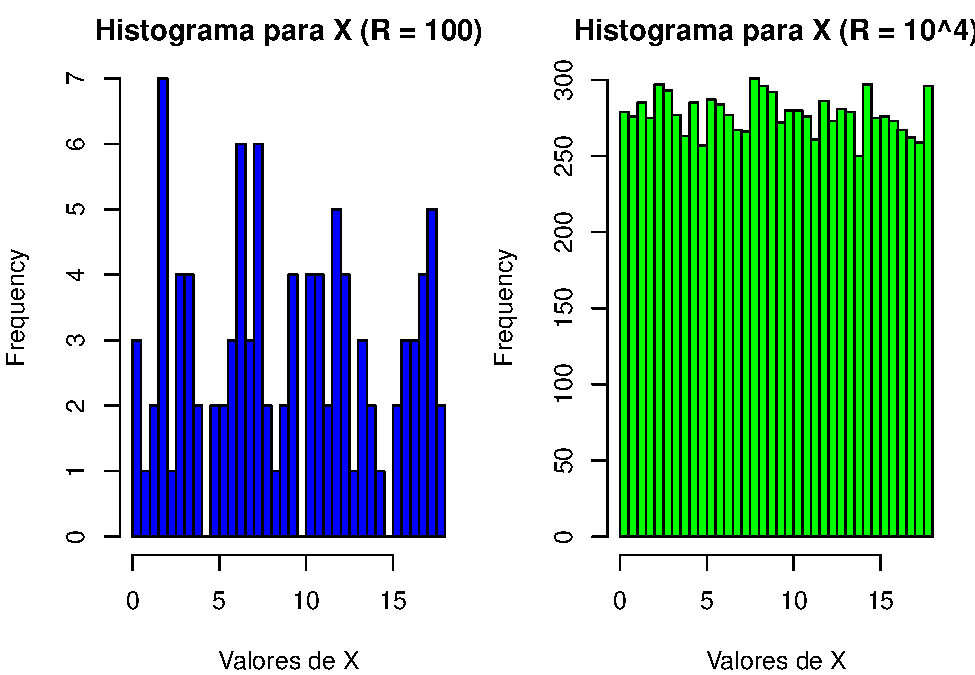
\includegraphics[keepaspectratio]{informe_files/figure-latex/unnamed-chunk-4-1.pdf}}

La distribución esperada es una distribución uniforme. Al aumentar el
número de realizaciones \(R\), el histograma se hace más suave y más
cercano a la densidad teórica de la distribución uniforme.

\section{Ejercicio 2: Otra Variable
Aleatoria}\label{ejercicio-2-otra-variable-aleatoria}

Dado que \(Y = \bar{X}_{15} = \frac{1}{15} \sum_{i=1}^{15} X_i\), donde
cada \(X_i\) es independiente e idénticamente distribuido
\(X_i \sim U(0, 18)\).

\subsection{\texorpdfstring{2.a Generar una función Y\_dist(R) que
devuelva un vector con \(R\) realizaciones de
\(Y\).}{2.a Generar una función Y\_dist(R) que devuelva un vector con R realizaciones de Y.}}\label{a-generar-una-funciuxf3n-y_distr-que-devuelva-un-vector-con-r-realizaciones-de-y.}

\begin{Shaded}
\begin{Highlighting}[]
\NormalTok{Y\_dist }\OtherTok{\textless{}{-}} \ControlFlowTok{function}\NormalTok{(R) \{}
\NormalTok{  realizaciones }\OtherTok{\textless{}{-}} \FunctionTok{replicate}\NormalTok{(R, }\FunctionTok{mean}\NormalTok{(}\FunctionTok{runif}\NormalTok{(}\DecValTok{15}\NormalTok{, }\AttributeTok{min =} \DecValTok{0}\NormalTok{, }\AttributeTok{max =} \DecValTok{18}\NormalTok{)))}
  \FunctionTok{return}\NormalTok{(realizaciones)}
\NormalTok{\}}
\end{Highlighting}
\end{Shaded}

\subsection{\texorpdfstring{2.b Calcular la media y la varianza muestral
de los datos para
\(R \in \{2, 30, 100, 10^4\}\).}{2.b Calcular la media y la varianza muestral de los datos para R \textbackslash in \textbackslash\{2, 30, 100, 10\^{}4\textbackslash\}.}}\label{b-calcular-la-media-y-la-varianza-muestral-de-los-datos-para-r-in-2-30-100-104.-1}

\begin{Shaded}
\begin{Highlighting}[]
\NormalTok{resultados\_Y }\OtherTok{\textless{}{-}} \FunctionTok{data.frame}\NormalTok{(}\AttributeTok{R =} \FunctionTok{integer}\NormalTok{(), }\AttributeTok{Media =} \FunctionTok{numeric}\NormalTok{(), }\AttributeTok{Varianza =} \FunctionTok{numeric}\NormalTok{())}

\ControlFlowTok{for}\NormalTok{ (R }\ControlFlowTok{in}\NormalTok{ R\_values) \{}
\NormalTok{  muestras\_Y }\OtherTok{\textless{}{-}} \FunctionTok{Y\_dist}\NormalTok{(R)}
\NormalTok{  media\_muestral\_Y }\OtherTok{\textless{}{-}} \FunctionTok{mean}\NormalTok{(muestras\_Y)}
\NormalTok{  varianza\_muestral\_Y }\OtherTok{\textless{}{-}} \FunctionTok{var}\NormalTok{(muestras\_Y)}
\NormalTok{  resultados\_Y }\OtherTok{\textless{}{-}} \FunctionTok{rbind}\NormalTok{(resultados\_Y, }\FunctionTok{data.frame}\NormalTok{(}\AttributeTok{R =}\NormalTok{ R, }\AttributeTok{Media =}\NormalTok{ media\_muestral\_Y, }\AttributeTok{Varianza =}\NormalTok{ varianza\_muestral\_Y))}
\NormalTok{\}}

\FunctionTok{print}\NormalTok{(resultados\_Y)}
\end{Highlighting}
\end{Shaded}

\begin{verbatim}
##       R    Media Varianza
## 1     2 8.427368 2.459774
## 2    30 8.954628 1.182842
## 3   100 9.124603 1.899916
## 4 10000 9.022645 1.766110
\end{verbatim}

\subsection{\texorpdfstring{2.c Comparar las medias empíricas y calcular
teóricamente \(E(Y)\) y
\(V(Y)\).}{2.c Comparar las medias empíricas y calcular teóricamente E(Y) y V(Y).}}\label{c-comparar-las-medias-empuxedricas-y-calcular-teuxf3ricamente-ey-y-vy.}

Teóricamente, \(E(Y) = E(X)\) y \(V(Y) = \frac{V(X)}{15}\).

\begin{Shaded}
\begin{Highlighting}[]
\NormalTok{E\_Y }\OtherTok{\textless{}{-}}\NormalTok{ E\_X  }\CommentTok{\# E(Y) = E(X)}
\NormalTok{V\_Y }\OtherTok{\textless{}{-}}\NormalTok{ V\_X }\SpecialCharTok{/} \DecValTok{15}  \CommentTok{\# V(Y) = V(X) / 15}

\FunctionTok{print}\NormalTok{(}\FunctionTok{paste}\NormalTok{(}\StringTok{"Esperanza E(Y):"}\NormalTok{, E\_Y))}
\end{Highlighting}
\end{Shaded}

\begin{verbatim}
## [1] "Esperanza E(Y): 9"
\end{verbatim}

\begin{Shaded}
\begin{Highlighting}[]
\FunctionTok{print}\NormalTok{(}\FunctionTok{paste}\NormalTok{(}\StringTok{"Varianza V(Y):"}\NormalTok{, V\_Y))}
\end{Highlighting}
\end{Shaded}

\begin{verbatim}
## [1] "Varianza V(Y): 1.8"
\end{verbatim}

Al comparar, notamos que:

\begin{itemize}
\tightlist
\item
  Las medias empíricas se aproximan bastante al valor esperado teórico
  \(E(Y)\).
\item
  La varianza muestral también se aproxima al valor teórico a medida que
  \(R\) aumenta.
\end{itemize}

\subsection{\texorpdfstring{2.d Hacer dos histogramas de \(Y\), tomando
\(R \in \{100, 10^4\}\) realizaciones y 30
bines.}{2.d Hacer dos histogramas de Y, tomando R \textbackslash in \textbackslash\{100, 10\^{}4\textbackslash\} realizaciones y 30 bines.}}\label{d-hacer-dos-histogramas-de-y-tomando-r-in-100-104-realizaciones-y-30-bines.}

\begin{Shaded}
\begin{Highlighting}[]
\FunctionTok{par}\NormalTok{(}\AttributeTok{mfrow =} \FunctionTok{c}\NormalTok{(}\DecValTok{1}\NormalTok{, }\DecValTok{2}\NormalTok{))  }\CommentTok{\# Configurar la ventana gráfica para dos gráficos lado a lado}
\FunctionTok{par}\NormalTok{(}\AttributeTok{mar =} \FunctionTok{c}\NormalTok{(}\DecValTok{4}\NormalTok{, }\DecValTok{4}\NormalTok{, }\DecValTok{2}\NormalTok{, }\DecValTok{1}\NormalTok{))  }\CommentTok{\# Ajustar los márgenes del gráfico}

\CommentTok{\# Histograma para R = 100}
\FunctionTok{hist}\NormalTok{(}\FunctionTok{Y\_dist}\NormalTok{(}\DecValTok{100}\NormalTok{), }\AttributeTok{breaks =} \DecValTok{30}\NormalTok{, }\AttributeTok{main =} \StringTok{"Histograma de Y (R = 100)"}\NormalTok{, }\AttributeTok{xlab =} \StringTok{"Y"}\NormalTok{, }\AttributeTok{col =} \StringTok{"magenta"}\NormalTok{)}

\CommentTok{\# Histograma para R = 10\^{}4}
\FunctionTok{hist}\NormalTok{(}\FunctionTok{Y\_dist}\NormalTok{(}\DecValTok{10}\SpecialCharTok{\^{}}\DecValTok{4}\NormalTok{), }\AttributeTok{breaks =} \DecValTok{30}\NormalTok{, }\AttributeTok{main =} \StringTok{"Histograma de Y (R = 10\^{}4)"}\NormalTok{, }\AttributeTok{xlab =} \StringTok{"Y"}\NormalTok{, }\AttributeTok{col =} \StringTok{"blue"}\NormalTok{)}
\end{Highlighting}
\end{Shaded}

\pandocbounded{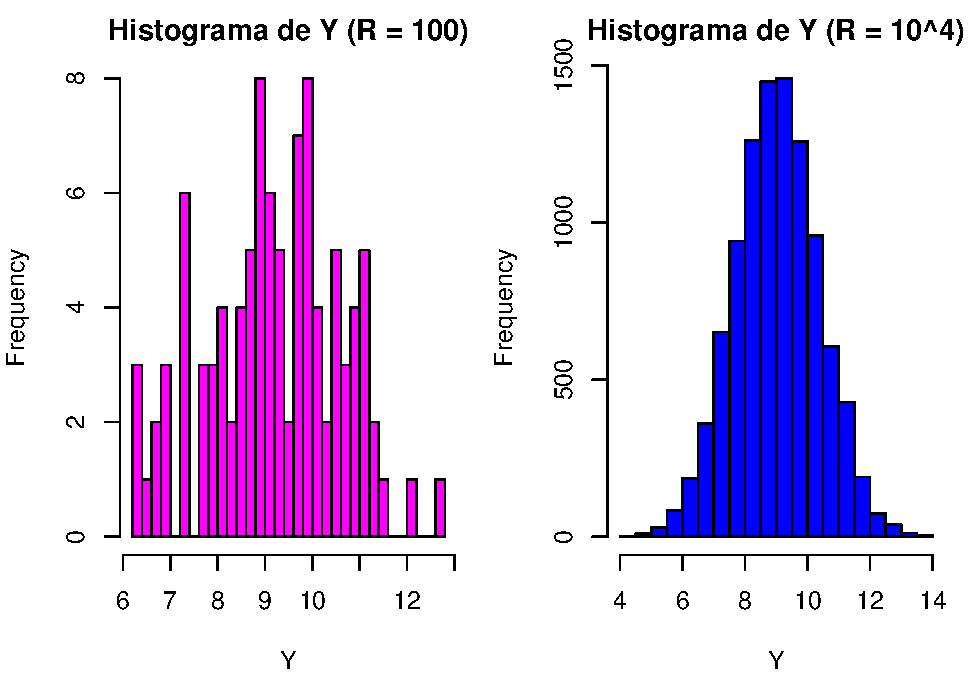
\includegraphics[keepaspectratio]{informe_files/figure-latex/unnamed-chunk-8-1.pdf}}

Esperamos ver una normal, tiene mucho menos dispersión que otro tipo de
distribuciones dado a que es simétrica. Los histogramas se parecen
porque hay menos varianza.

\section{Ejercicio 3: Teorema Central del
Límite}\label{ejercicio-3-teorema-central-del-luxedmite}

\subsection{3.a Mostrar que se cumple el TCL para un caso
particular}\label{a-mostrar-que-se-cumple-el-tcl-para-un-caso-particular}

Generamos un histograma para \(X\) y otro para \(X_{40}\), ambos con
\(R = 10^6\) realizaciones.

\begin{Shaded}
\begin{Highlighting}[]
\NormalTok{R }\OtherTok{\textless{}{-}} \DecValTok{10}\SpecialCharTok{\^{}}\DecValTok{6}
\NormalTok{n }\OtherTok{\textless{}{-}} \DecValTok{40}

\NormalTok{X }\OtherTok{\textless{}{-}} \FunctionTok{runif}\NormalTok{(R, }\AttributeTok{min =} \DecValTok{0}\NormalTok{, }\AttributeTok{max =} \DecValTok{18}\NormalTok{)}
\NormalTok{X\_40 }\OtherTok{\textless{}{-}} \FunctionTok{replicate}\NormalTok{(R, }\FunctionTok{mean}\NormalTok{(}\FunctionTok{runif}\NormalTok{(n, }\AttributeTok{min =} \DecValTok{0}\NormalTok{, }\AttributeTok{max =} \DecValTok{18}\NormalTok{)))}

\FunctionTok{par}\NormalTok{(}\AttributeTok{mfrow =} \FunctionTok{c}\NormalTok{(}\DecValTok{1}\NormalTok{, }\DecValTok{2}\NormalTok{))}
\FunctionTok{par}\NormalTok{(}\AttributeTok{mar =} \FunctionTok{c}\NormalTok{(}\DecValTok{4}\NormalTok{, }\DecValTok{4}\NormalTok{, }\DecValTok{2}\NormalTok{, }\DecValTok{1}\NormalTok{))  }\CommentTok{\# Ajustar los márgenes del gráfico}

\CommentTok{\# Histograma para X}
\FunctionTok{hist}\NormalTok{(X, }\AttributeTok{breaks =} \DecValTok{50}\NormalTok{, }\AttributeTok{probability =} \ConstantTok{TRUE}\NormalTok{, }\AttributeTok{main =} \StringTok{"Histograma de X"}\NormalTok{, }\AttributeTok{xlab =} \StringTok{"X"}\NormalTok{, }\AttributeTok{col =} \StringTok{"lightblue"}\NormalTok{)}
\FunctionTok{curve}\NormalTok{(}\FunctionTok{dunif}\NormalTok{(x, }\AttributeTok{min =} \DecValTok{0}\NormalTok{, }\AttributeTok{max =} \DecValTok{18}\NormalTok{), }\AttributeTok{col =} \StringTok{"red"}\NormalTok{, }\AttributeTok{lwd =} \DecValTok{2}\NormalTok{, }\AttributeTok{add =} \ConstantTok{TRUE}\NormalTok{)}

\CommentTok{\# Histograma para X\_40}
\FunctionTok{hist}\NormalTok{(X\_40, }\AttributeTok{breaks =} \DecValTok{50}\NormalTok{, }\AttributeTok{probability =} \ConstantTok{TRUE}\NormalTok{, }\AttributeTok{main =} \StringTok{"Histograma de X\_40"}\NormalTok{, }\AttributeTok{xlab =} \StringTok{"X\_40"}\NormalTok{, }\AttributeTok{col =} \StringTok{"lightgreen"}\NormalTok{)}
\NormalTok{mu }\OtherTok{\textless{}{-}} \DecValTok{9}  \CommentTok{\# Esperanza de X}
\NormalTok{sigma }\OtherTok{\textless{}{-}} \FunctionTok{sqrt}\NormalTok{((}\DecValTok{18} \SpecialCharTok{{-}} \DecValTok{0}\NormalTok{)}\SpecialCharTok{\^{}}\DecValTok{2} \SpecialCharTok{/} \DecValTok{12}\NormalTok{) }\SpecialCharTok{/} \FunctionTok{sqrt}\NormalTok{(n)  }
\FunctionTok{curve}\NormalTok{(}\FunctionTok{dnorm}\NormalTok{(x, }\AttributeTok{mean =}\NormalTok{ mu, }\AttributeTok{sd =}\NormalTok{ sigma), }\AttributeTok{col =} \StringTok{"red"}\NormalTok{, }\AttributeTok{lwd =} \DecValTok{2}\NormalTok{, }\AttributeTok{add =} \ConstantTok{TRUE}\NormalTok{)}
\end{Highlighting}
\end{Shaded}

\pandocbounded{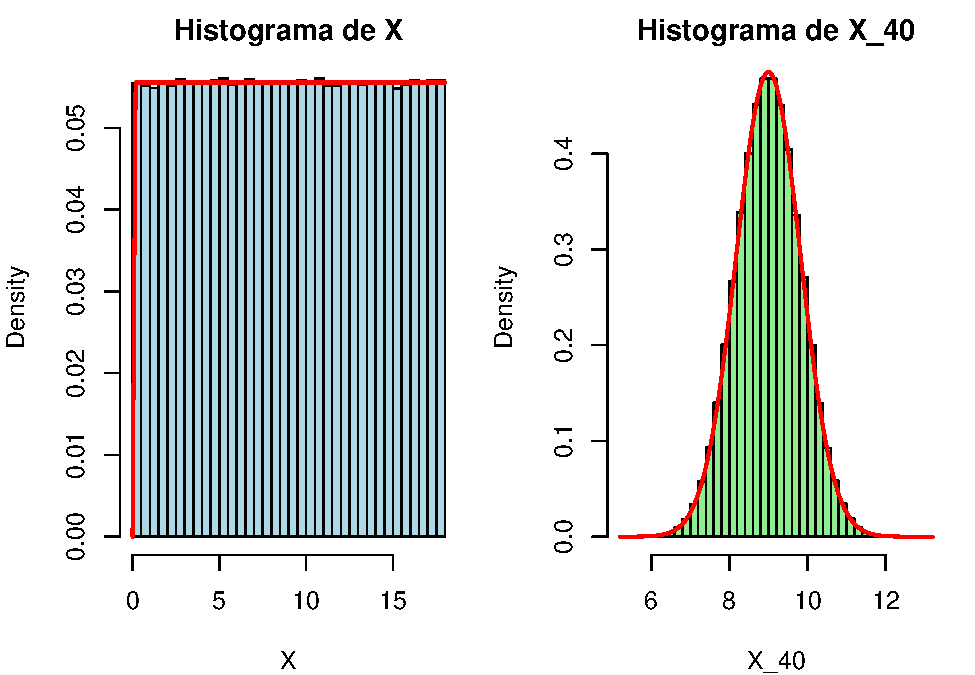
\includegraphics[keepaspectratio]{informe_files/figure-latex/unnamed-chunk-9-1.pdf}}

\subsection{3.b Graficar ocho histogramas en un arreglo de 4x2
paneles}\label{b-graficar-ocho-histogramas-en-un-arreglo-de-4x2-paneles}

Se varía el número de realizaciones \(n \in \{1, 2, 5, 15\}\) y el
número de simulaciones \(R \in \{10^2, 10^6\}\).

\begin{Shaded}
\begin{Highlighting}[]
\NormalTok{n\_values }\OtherTok{\textless{}{-}} \FunctionTok{c}\NormalTok{(}\DecValTok{1}\NormalTok{, }\DecValTok{2}\NormalTok{, }\DecValTok{5}\NormalTok{, }\DecValTok{15}\NormalTok{)}
\NormalTok{R\_values }\OtherTok{\textless{}{-}} \FunctionTok{c}\NormalTok{(}\DecValTok{10}\SpecialCharTok{\^{}}\DecValTok{2}\NormalTok{, }\DecValTok{10}\SpecialCharTok{\^{}}\DecValTok{6}\NormalTok{)}

\FunctionTok{par}\NormalTok{(}\AttributeTok{mfrow =} \FunctionTok{c}\NormalTok{(}\DecValTok{2}\NormalTok{, }\DecValTok{2}\NormalTok{))  }\CommentTok{\# Reducir a 4 gráficos por página para dar más espacio a cada uno}
\FunctionTok{par}\NormalTok{(}\AttributeTok{mar =} \FunctionTok{c}\NormalTok{(}\DecValTok{4}\NormalTok{, }\DecValTok{4}\NormalTok{, }\DecValTok{2}\NormalTok{, }\DecValTok{1}\NormalTok{))  }\CommentTok{\# Ajustar los márgenes del gráfico}

\ControlFlowTok{for}\NormalTok{ (n }\ControlFlowTok{in}\NormalTok{ n\_values) \{}
  \ControlFlowTok{for}\NormalTok{ (R }\ControlFlowTok{in}\NormalTok{ R\_values) \{}
\NormalTok{    X\_n }\OtherTok{\textless{}{-}} \FunctionTok{replicate}\NormalTok{(R}

\NormalTok{, }\FunctionTok{mean}\NormalTok{(}\FunctionTok{runif}\NormalTok{(n, }\AttributeTok{min =} \DecValTok{0}\NormalTok{, }\AttributeTok{max =} \DecValTok{18}\NormalTok{)))}
    \FunctionTok{hist}\NormalTok{(X\_n, }\AttributeTok{breaks =} \DecValTok{50}\NormalTok{, }\AttributeTok{probability =} \ConstantTok{TRUE}\NormalTok{,}
         \AttributeTok{main =} \FunctionTok{paste}\NormalTok{(}\StringTok{"n ="}\NormalTok{, n, }\StringTok{", R ="}\NormalTok{, R),}
         \AttributeTok{xlab =} \StringTok{"X\_n"}\NormalTok{, }\AttributeTok{col =} \StringTok{"lightgray"}\NormalTok{)}
    
    \ControlFlowTok{if}\NormalTok{ (n }\SpecialCharTok{\textgreater{}} \DecValTok{1}\NormalTok{) \{}
\NormalTok{      mu }\OtherTok{\textless{}{-}} \DecValTok{9}  \CommentTok{\# Esperanza de X}
\NormalTok{      sigma }\OtherTok{\textless{}{-}} \FunctionTok{sqrt}\NormalTok{((}\DecValTok{18} \SpecialCharTok{{-}} \DecValTok{0}\NormalTok{)}\SpecialCharTok{\^{}}\DecValTok{2} \SpecialCharTok{/} \DecValTok{12}\NormalTok{) }\SpecialCharTok{/} \FunctionTok{sqrt}\NormalTok{(n)  }
      \FunctionTok{curve}\NormalTok{(}\FunctionTok{dnorm}\NormalTok{(x, }\AttributeTok{mean =}\NormalTok{ mu, }\AttributeTok{sd =}\NormalTok{ sigma), }\AttributeTok{col =} \StringTok{"red"}\NormalTok{, }\AttributeTok{lwd =} \DecValTok{2}\NormalTok{, }\AttributeTok{add =} \ConstantTok{TRUE}\NormalTok{)}
\NormalTok{    \}}
\NormalTok{  \}}
\NormalTok{\}}
\end{Highlighting}
\end{Shaded}

\pandocbounded{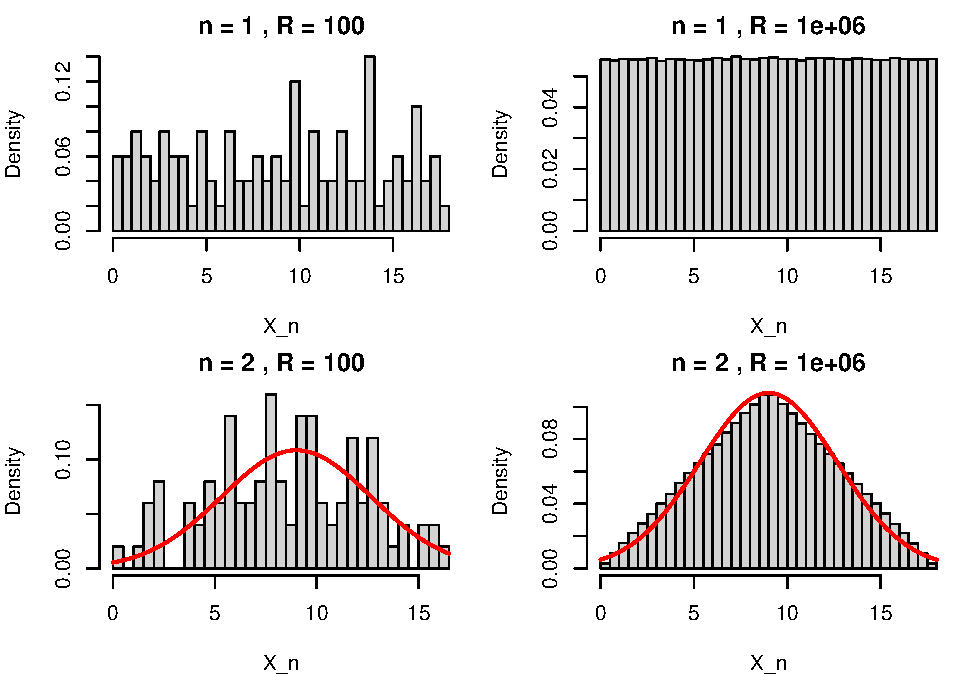
\includegraphics[keepaspectratio]{informe_files/figure-latex/unnamed-chunk-10-1.pdf}}
\pandocbounded{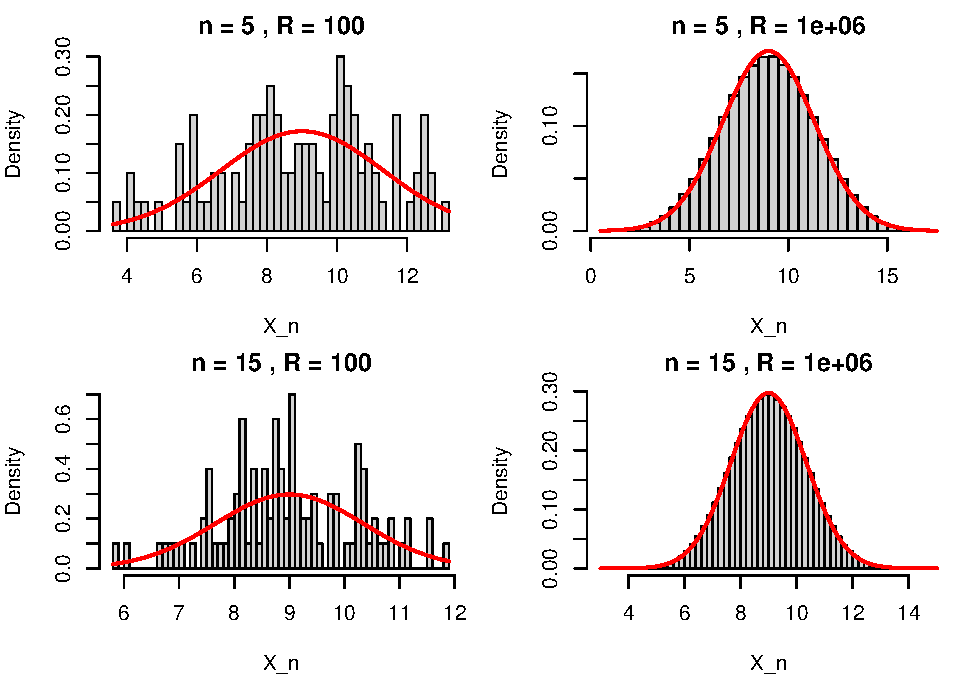
\includegraphics[keepaspectratio]{informe_files/figure-latex/unnamed-chunk-10-2.pdf}}

Sabemos que si modificamos la variable R, la distribución no cambiará.
Simplemente mostrará más o menos sampleos de la misma distribución, más
o menos definida, dependiendo de la cantidad de datos. En cambio, al
variar \(n\), el valor promedio de las muestras se acerca cada vez más a
la esperanza teórica de la variable aleatoria subyacente, como se espera
según el Teorema Central del Límite (TCL) y la Ley de los Grandes
Números.

\end{document}
